\documentclass[10pt,a4paper]{article}
\usepackage[T1]{fontenc}
\usepackage{lmodern}
\usepackage[margin=1.8cm]{geometry}
\usepackage{booktabs}
\usepackage{tabularx}
\usepackage{array}
\usepackage{graphicx}
\usepackage{xcolor}
\usepackage{amsmath}
\usepackage{enumitem}
\usepackage{fancyhdr}
\usepackage[hidelinks]{hyperref}
\usepackage{caption}
\usepackage{float}

\definecolor{Navy}{HTML}{17324D}
\definecolor{Green}{HTML}{147A5B}
\definecolor{Gold}{HTML}{D49B2A}
\definecolor{Light}{HTML}{F1F4F6}
\definecolor{Gray}{HTML}{667788}
\definecolor{Red}{HTML}{B54242}

\hypersetup{colorlinks=true,linkcolor=Navy,urlcolor=Green}
\setlength{\parindent}{0pt}
\setlength{\parskip}{5pt}
\setlist[itemize]{leftmargin=1.3em,itemsep=2pt,topsep=2pt}
\setlist[enumerate]{leftmargin=1.5em,itemsep=2pt,topsep=2pt}
\renewcommand{\arraystretch}{1.15}
\newcolumntype{L}[1]{>{\raggedright\arraybackslash}p{#1}}
\newcolumntype{Y}{>{\raggedright\arraybackslash}X}

\pagestyle{fancy}
\fancyhf{}
\lhead{\color{Gray}\small TSP free-acid modeling}
\rhead{\color{Gray}\small Project progress}
\cfoot{\color{Gray}\small \thepage}
\renewcommand{\headrulewidth}{0.3pt}

\newcommand{\good}[1]{\textcolor{Green}{\textbf{#1}}}
\newcommand{\bad}[1]{\textcolor{Red}{\textbf{#1}}}
\newcommand{\pending}[1]{\textcolor{Gold}{\textbf{#1}}}
\newcommand{\statusbox}[1]{\colorbox{Light}{\parbox{0.96\linewidth}{#1}}}

\begin{document}

\begin{titlepage}
  \color{Navy}
  \vspace*{2.4cm}
  {\Huge\bfseries SLURRY\_FREE\_ACID Modeling\par}
  \vspace{0.3cm}
  {\LARGE Project Advancement Report\par}
  \vspace{0.8cm}
  {\large Data preparation, forecasting benchmarks, virtual sensing, and dashboard\par}
  \vspace{0.8cm}
  {\large Done by : Benfellah ikram}
  \vfill
  \statusbox{\textbf{Current result:} the target-anchored change model beats persistence at all four horizons. I also built a separate target-free virtual sensor for process-only data. The next required test is validation on another month.}
  \vfill
 
  {\large Internship project\hfill}
  \vspace{0.3cm}
  \color{Gold}\rule{\textwidth}{4pt}
\end{titlepage}

\section*{Executive summary}

I completed the following work:
\begin{itemize}
  \item explored and checked one month of one-minute process data;
  \item prepared four forecast horizons and four feature-set hypotheses;
  \item benchmarked direct future-level prediction against persistence;
  \item improved forecasting by predicting the future target change;
  \item built a separate target-free virtual sensor;
  \item integrated the results into an interactive dashboard.
\end{itemize}

I kept three operational cases separate because their input requirements are different.

\begin{tabularx}{\textwidth}{L{0.20\textwidth}Y Y}
\toprule
\textbf{Case} & \textbf{Prediction contract} & \textbf{Executed result} \\
\midrule
Direct future level & Process measurements at or before $t$ predict $y_{t+h}$. & Learned the operating level but did not beat persistence. \\
Target-anchored forecast & Process and target history predict $\Delta y_{t,h}$; reconstruct $\hat y_{t+h}=y_t+\widehat{\Delta y}_{t,h}$. & Ridge with the hybrid full set beat persistence by 19.8--34.9\%. \\
Target-free virtual sensor & Process measurements only predict the current $y_t$. & Ridge--LightGBM blend achieved test RMSE 0.301 and $R^2=0.558$. \\
\bottomrule
\end{tabularx}

\textbf{Current decision}
\begin{itemize}
  \item Use the target-anchored model when the current free-acid value is available.
  \item Use the virtual sensor for process-only data; it estimates the current value, not a future warning.
  \item Do not consider either model operationally validated until it is tested on another month.
\end{itemize}

\section{Scope and data}

\begin{tabularx}{\textwidth}{L{0.28\textwidth}Y}
\toprule
\textbf{Item} & \textbf{Executed scope} \\
\midrule
Dataset & 44,640 one-minute observations covering 31 days in January 2026 \\
Inputs & 21 original process measurements \\
Target & \texttt{SLURRY\_FREE\_ACID} \\
Forecast horizons & 1, 5, 10, and 15 minutes \\
Split policy & First 70\% training, next 15\% validation, final 15\% test; no shuffle \\
Selection policy & Preprocessing, lag selection, filtering, hyperparameters, and blend weights selected without test fitting \\
Main benchmark & Persistence: $\hat y_{t+h}=y_t$ whenever the current target is available \\
\bottomrule
\end{tabularx}

\textbf{Why chronological splitting:} adjacent one-minute rows are dependent. Random splitting could place almost identical neighboring states in training and test and give overly optimistic results.

\section{Work completed by notebook}

\begin{tabularx}{\textwidth}{L{0.10\textwidth}L{0.28\textwidth}Y}
\toprule
\textbf{Notebook} & \textbf{Purpose} & \textbf{Completed output} \\
\midrule
01 & Data exploration & Timestamp, missingness, target behavior, sensor relationships, delayed behavior, and unusual-period assessment. \\
02 & Feature preparation & Four horizons, process registry, selected lags, compact temporal and process-aware features, four feature sets, chronological splits, train-fitted preprocessing, and audit artifacts. \\
03 & Direct benchmark & Mean and persistence baselines; Ridge, Extra Trees, and histogram gradient boosting across all 16 horizon/feature-set configurations. \\
04 & Delta and transition study & Delta regression, target-history ablation, transition weighting, warning classification, regime errors, feature importance, and fitted research candidates. \\
05 & Target-free virtual sensor & Process-only baselines, seven model families, validation-selected blend, drift diagnostics, empirical intervals, and saved inference bundle. \\
Dashboard & Interactive delivery & CSV upload, exploration, transition-window investigation, target-anchored forecasts, target-free estimates, drift flags, and label-dependent evaluation. \\
\bottomrule
\end{tabularx}

\section{Feature-preparation methodology}

\begin{figure}[H]
\centering
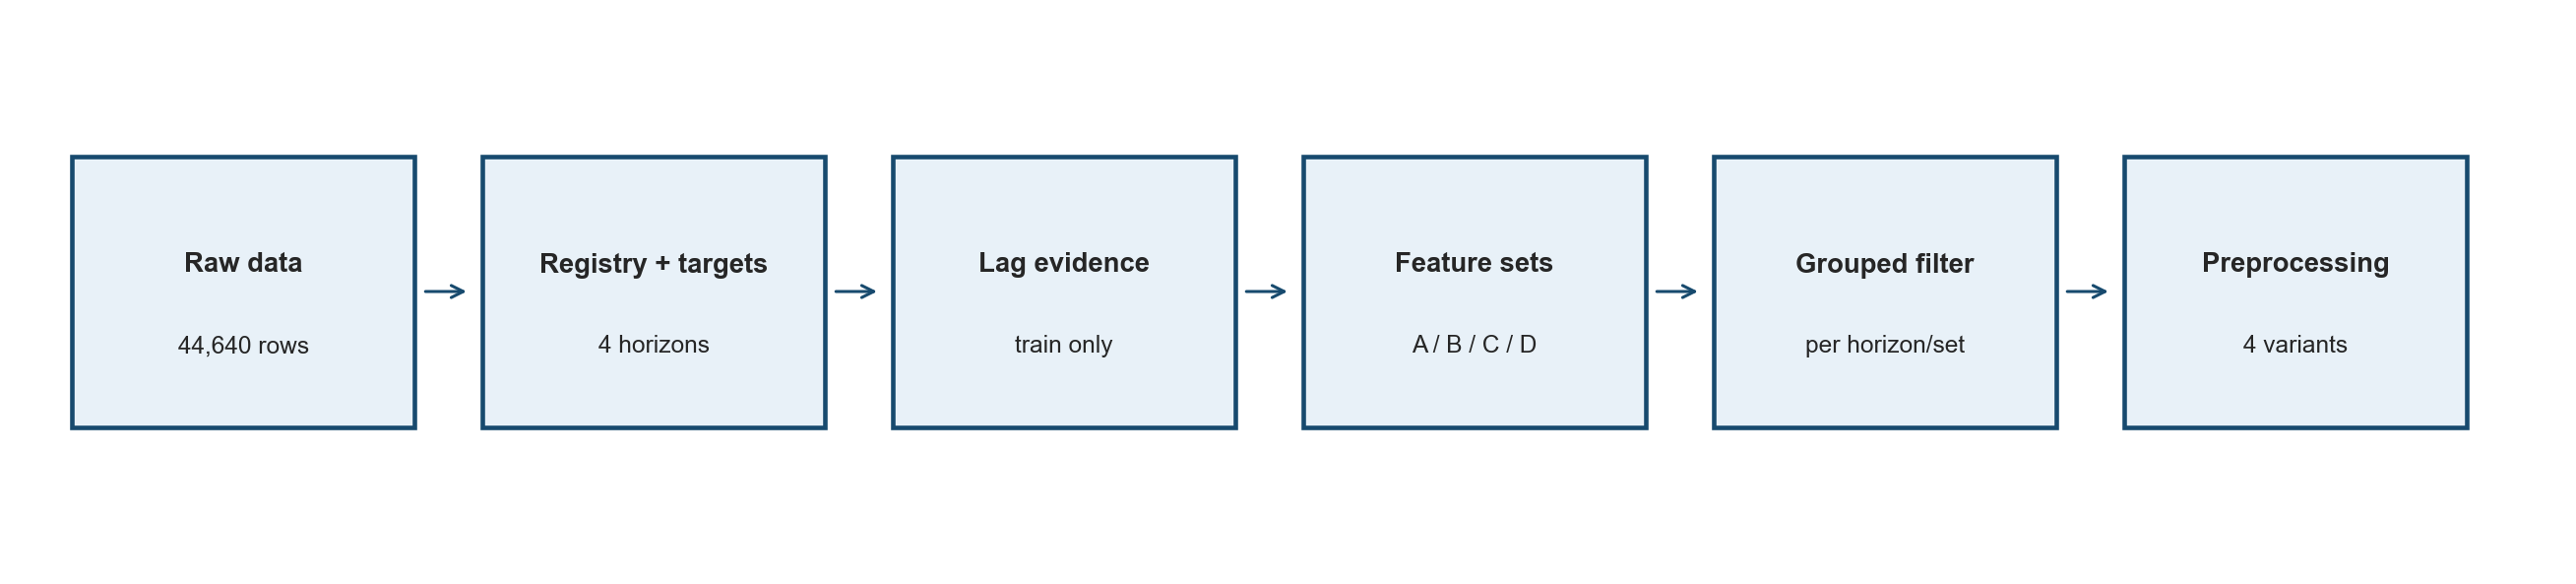
\includegraphics[width=\textwidth]{feature_preparation_artifacts/figures/pipeline_overview.png}
\caption{Executed feature-preparation pipeline. Every statistical decision that can leak target information is restricted to training data.}
\end{figure}

\subsection*{Targets and leakage controls}

I created the direct targets:
\[
y_{t+h}=\texttt{SLURRY\_FREE\_ACID}_{t+h},
\qquad h\in\{1,5,10,15\}.
\]
\begin{itemize}
  \item Every input at timestamp $t$ uses data from $t$ or earlier.
  \item I removed the first 30 rows because their required history does not exist.
  \item Later sensor gaps receive missingness indicators and training-median imputation.
\end{itemize}

\subsection*{Training-only lag selection}

I tested lags of 1, 5, 10, 15, 30, and 60 minutes and retained at most three per sensor using:
\begin{itemize}
  \item absolute lagged correlation with the one-minute future target;
  \item mutual information;
  \item sign and magnitude stability across three chronological training blocks;
  \item a 0.15 score bonus for a process-response prior.
\end{itemize}
I then added two rolling means, one rolling standard deviation, a five-minute difference, and a ten-minute slope per source variable.

\subsection*{Process-aware engineering}

I added:
\begin{itemize}
  \item total acid flow and acid-line imbalance;
  \item acid-to-phosphate ratio;
  \item confirmed total slurry volumetric flow;
  \item slurry-density proxy;
  \item thermal gradients and a steam-condition proxy;
  \item drying-intensity and recycle-to-production proxies;
  \item flow coefficients of variation.
\end{itemize}

\textbf{Validation boundary}
\begin{itemize}
  \item Total slurry volumetric flow is confirmed as the sum of the two $m^3/h$ signals.
  \item Total acid flow is confirmed additive, but its unit remains unresolved.
  \item Density, energy, drying, and recycle features remain proxies, not verified physical quantities.
\end{itemize}

Numerically risky process features use $\epsilon=10^{-6}$, replace infinities with missing values, and are clipped using the training-period 0.1th and 99.9th percentiles.

\subsection*{Feature-set hypotheses and final dimensions}

\begin{tabularx}{\textwidth}{L{0.15\textwidth}Y L{0.16\textwidth}L{0.14\textwidth}}
\toprule
\textbf{Set} & \textbf{Hypothesis} & \textbf{Candidates} & \textbf{Retained} \\
\midrule
A -- Raw & Current measurements may be sufficient. & 21 & 21 \\
B -- Temporal & Selected histories and recent dynamics add information. & 210 & 162 \\
C -- Process-aware & Interpretable balances, ratios, gradients, and stability measures add information. & 58 & 58 \\
D -- Full & Temporal and process-relationship evidence are complementary. & 226 & 178 \\
\bottomrule
\end{tabularx}

\textbf{Correlation filtering}
\begin{itemize}
  \item Applied inside each original-sensor family at $|r|>0.98$ using training data only.
  \item Priority: raw value, selected lag, rolling mean, difference, slope, then variability.
  \item Process-aware features and missingness indicators are protected from blanket removal.
\end{itemize}

\section{Model training and selection}

\subsection*{Controlled model families}

\begin{tabularx}{\textwidth}{L{0.19\textwidth}Y Y}
\toprule
\textbf{Model} & \textbf{Role} & \textbf{Main executed choices} \\
\midrule
Ridge & Regularized linear reference for correlated features & Standard scaling; $\alpha\in\{1,10\}$ \\
PLS & Industrial latent-variable soft-sensor reference & 5 or 10 components; pre-standardized inputs \\
KNN & Local historical-state hypothesis & 25 or 75 distance-weighted neighbors \\
Extra Trees & Nonlinear thresholds and interactions & 30--60 trees; leaf-size and feature-fraction alternatives \\
HistGradient & Efficient nonlinear boosting & 50--80 iterations; controlled learning rates and leaf counts \\
XGBoost & Regularized boosted-tree reference & 150 trees; depths 4 or 6; row and feature subsampling 0.8 \\
LightGBM & Leaf-wise boosted-tree reference & 150 trees; 15 or 31 leaves; minimum child size 40 \\
Weighted blend & Complementary linear and nonlinear errors & Validation grid in 0.1 weight increments \\
\bottomrule
\end{tabularx}

\textbf{Selection procedure}
\begin{enumerate}
  \item Fit each candidate on training data.
  \item Rank candidates using validation RMSE.
  \item Keep the lowest-validation-RMSE candidate.
  \item Evaluate it once on the untouched test period.
\end{enumerate}
I did not select models using test performance. The reported test models were not refitted on training plus validation.

\section{Direct future-level benchmark}

The first experiment learned
\[
X_{\leq t}\longrightarrow \hat y_{t+h}.
\]
Validation selected Feature Set D with Ridge at every horizon.

\begin{table}[ht]
\centering
\begin{tabular}{rrrrr}
\toprule
\textbf{Horizon} & \textbf{MAE} & \textbf{RMSE} & \textbf{$R^2$} & \textbf{vs. persistence} \\
\midrule
1 min & 0.269 & 0.332 & 0.465 & \bad{-67.9\%} \\
5 min & 0.275 & 0.338 & 0.445 & \bad{-35.1\%} \\
10 min & 0.280 & 0.344 & 0.426 & \bad{-22.6\%} \\
15 min & 0.304 & 0.378 & 0.306 & \bad{-27.5\%} \\
\bottomrule
\end{tabular}
\caption{Untouched test performance for the validation-selected direct-level model. Negative improvement means worse than persistence.}
\end{table}

\textbf{Conclusion}
\begin{itemize}
  \item The model learned the broad operating level.
  \item It remained worse than carrying the current target forward.
  \item I therefore changed the task from predicting the level to predicting its future movement.
\end{itemize}

\section{Target-anchored change forecasting}

I reframed the task as:
\[
\Delta y_{t,h}=y_{t+h}-y_t,
\qquad
\hat y_{t+h}=y_t+\widehat{\Delta y}_{t,h}.
\]
I compared four input families:
\begin{itemize}
  \item 21 raw process measurements;
  \item 178 full exogenous features;
  \item 10 current/past target-history features;
  \item a 188-feature hybrid of full process information and target history.
\end{itemize}
Ridge and Extra Trees received equal two-candidate tuning budgets. Validation selected the 188-feature hybrid Ridge with $\alpha=10$ at every horizon.

\begin{table}[ht]
\centering
\begin{tabular}{rrrrr}
\toprule
\textbf{Horizon} & \textbf{MAE} & \textbf{RMSE} & \textbf{$R^2$} & \textbf{vs. persistence} \\
\midrule
1 min & 0.102 & 0.151 & 0.889 & \good{+23.2\%} \\
5 min & 0.113 & 0.169 & 0.862 & \good{+32.3\%} \\
10 min & 0.126 & 0.182 & 0.839 & \good{+34.9\%} \\
15 min & 0.176 & 0.237 & 0.726 & \good{+19.8\%} \\
\bottomrule
\end{tabular}
\caption{Untouched test performance after future-level reconstruction.}
\end{table}

\begin{figure}[H]
\centering
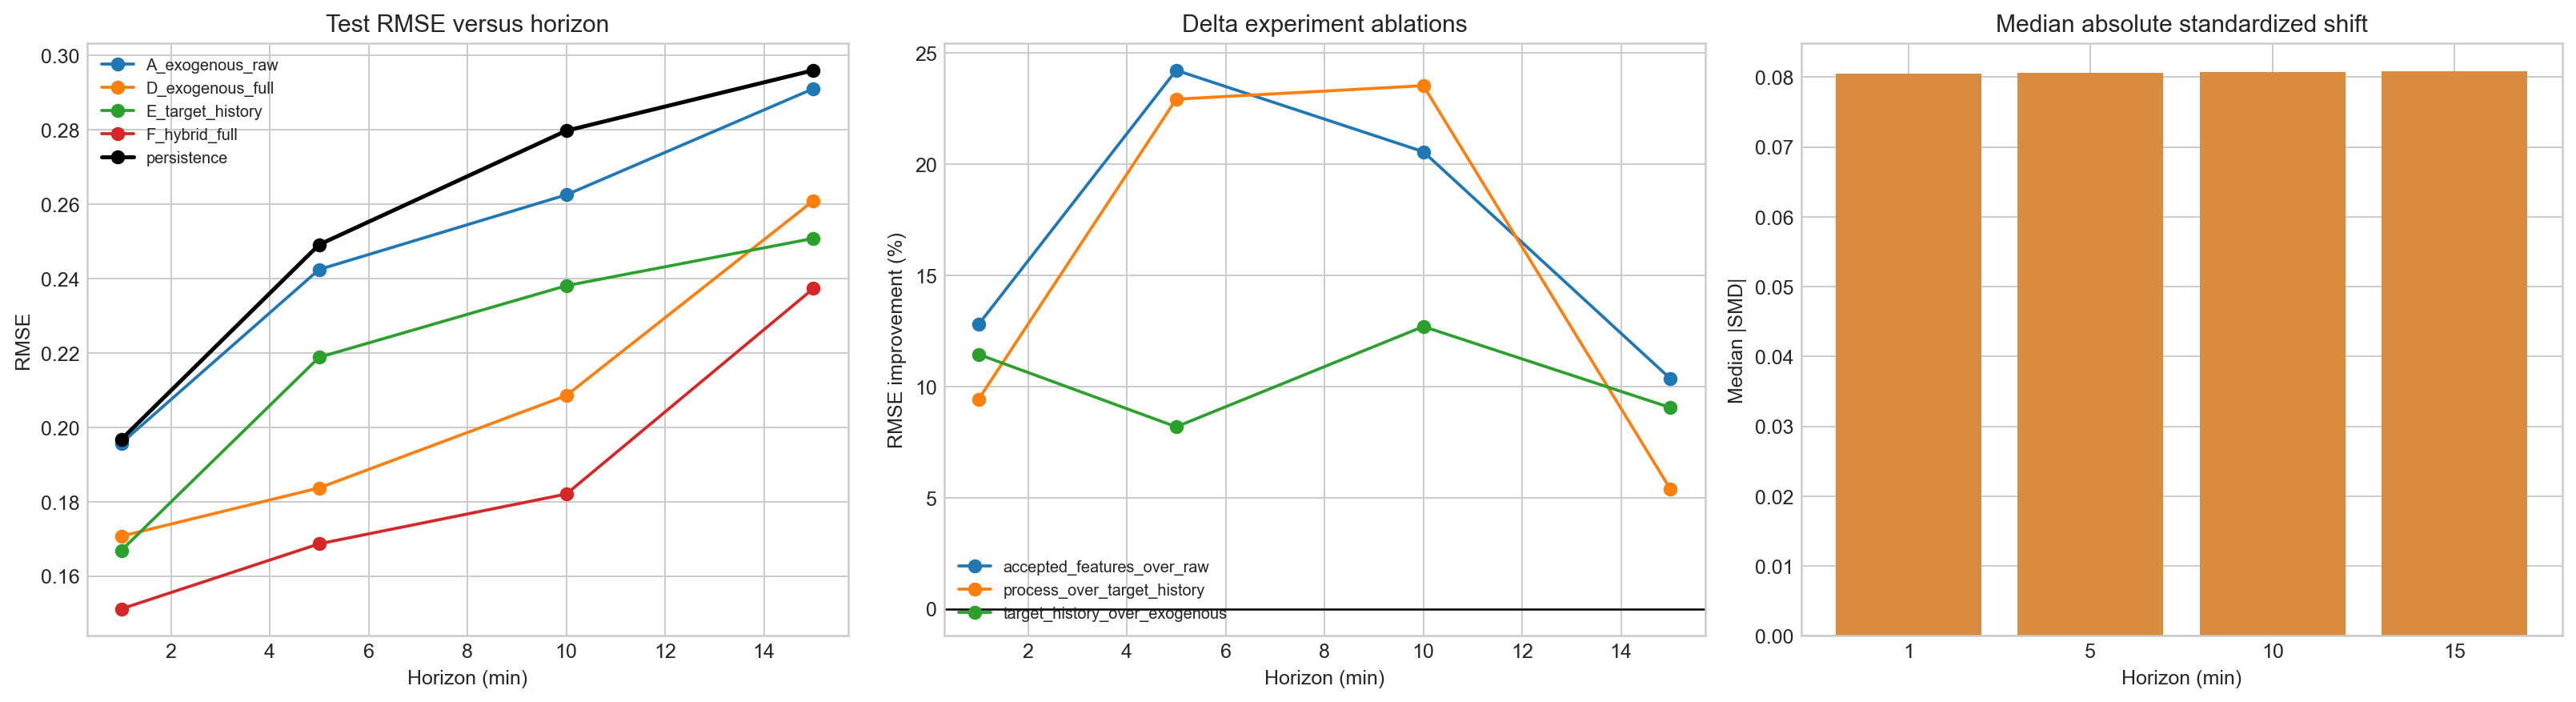
\includegraphics[width=\textwidth]{delta_transition_artifacts/figures/delta_performance_ablation_and_shift.png}
\caption{Delta performance, ablation gains, and standardized distribution shift. The hybrid full experiment gives the lowest RMSE across horizons.}
\end{figure}

\textbf{Ablation evidence.}
\begin{itemize}
  \item Accepted engineered features improved over raw process inputs by 10.3--24.2\%, depending on horizon.
  \item Target history improved over exogenous full inputs by 8.2--12.7\%.
  \item Process/full information improved over target history alone by 5.4--23.5\%.
\end{itemize}

\begin{itemize}
  \item One minute gives the lowest absolute error.
  \item Ten minutes gives the largest relative improvement over persistence.
  \item The final horizon must be chosen using both error and required reaction time.
\end{itemize}

\subsection*{Transition and warning experiments}

\begin{itemize}
  \item Candidate transitions use the training 90th percentile of $|\Delta y_{t,h}|$.
  \item Extreme candidates use the 95th percentile.
  \item These are statistical labels, not confirmed plant events.
  \item Giving transition rows four times the training weight slightly improved some transition errors but worsened overall RMSE, so I did not retain that model.
\end{itemize}

\begin{tabular}{rrrrr}
\toprule
\textbf{Horizon} & \textbf{Precision} & \textbf{Recall} & \textbf{F1} & \textbf{False-warning rate} \\
\midrule
1 min & 0.141 & 0.478 & 0.218 & 0.288 \\
5 min & 0.155 & 0.491 & 0.235 & 0.264 \\
10 min & 0.161 & 0.512 & 0.245 & 0.267 \\
15 min & 0.142 & 0.404 & 0.210 & 0.259 \\
\bottomrule
\end{tabular}

\textbf{Decision:} I kept the logistic transition classifier as a diagnostic only. Its precision is too low and its false-warning rate is too high for an operational alarm.

\section{Target-free virtual sensor}

The third case estimates the current target without target input:
\[
X_{\leq t}\longrightarrow \hat y_t.
\]
\begin{itemize}
  \item Inputs: the 21 original process measurements and accepted Notebook 02 derivatives.
  \item Forbidden inputs: current target, target history, and future-target columns.
  \item Comparison: 14 experiments covering seven model families and two feature sets.
\end{itemize}
Validation selected the two-member blend:
\[
\hat y_t=0.5\hat y_t^{\text{Ridge,D}}
+0.5\hat y_t^{\text{LightGBM,D}}.
\]

\begin{table}[ht]
\centering
\begin{tabular}{lrr}
\toprule
\textbf{Test metric} & \textbf{Training-mean baseline} & \textbf{Selected blend} \\
\midrule
MAE & 0.355 & \good{0.249} \\
RMSE & 0.454 & \good{0.301} \\
$R^2$ & approximately 0 & \good{0.558} \\
Median absolute error & -- & 0.229 \\
90th-percentile absolute error & -- & 0.459 \\
95th-percentile absolute error & -- & 0.536 \\
\bottomrule
\end{tabular}
\caption{Target-free current-time soft-sensor performance. RMSE improves by approximately 33.6\% over the training-mean baseline.}
\end{table}

\begin{figure}[H]
\centering
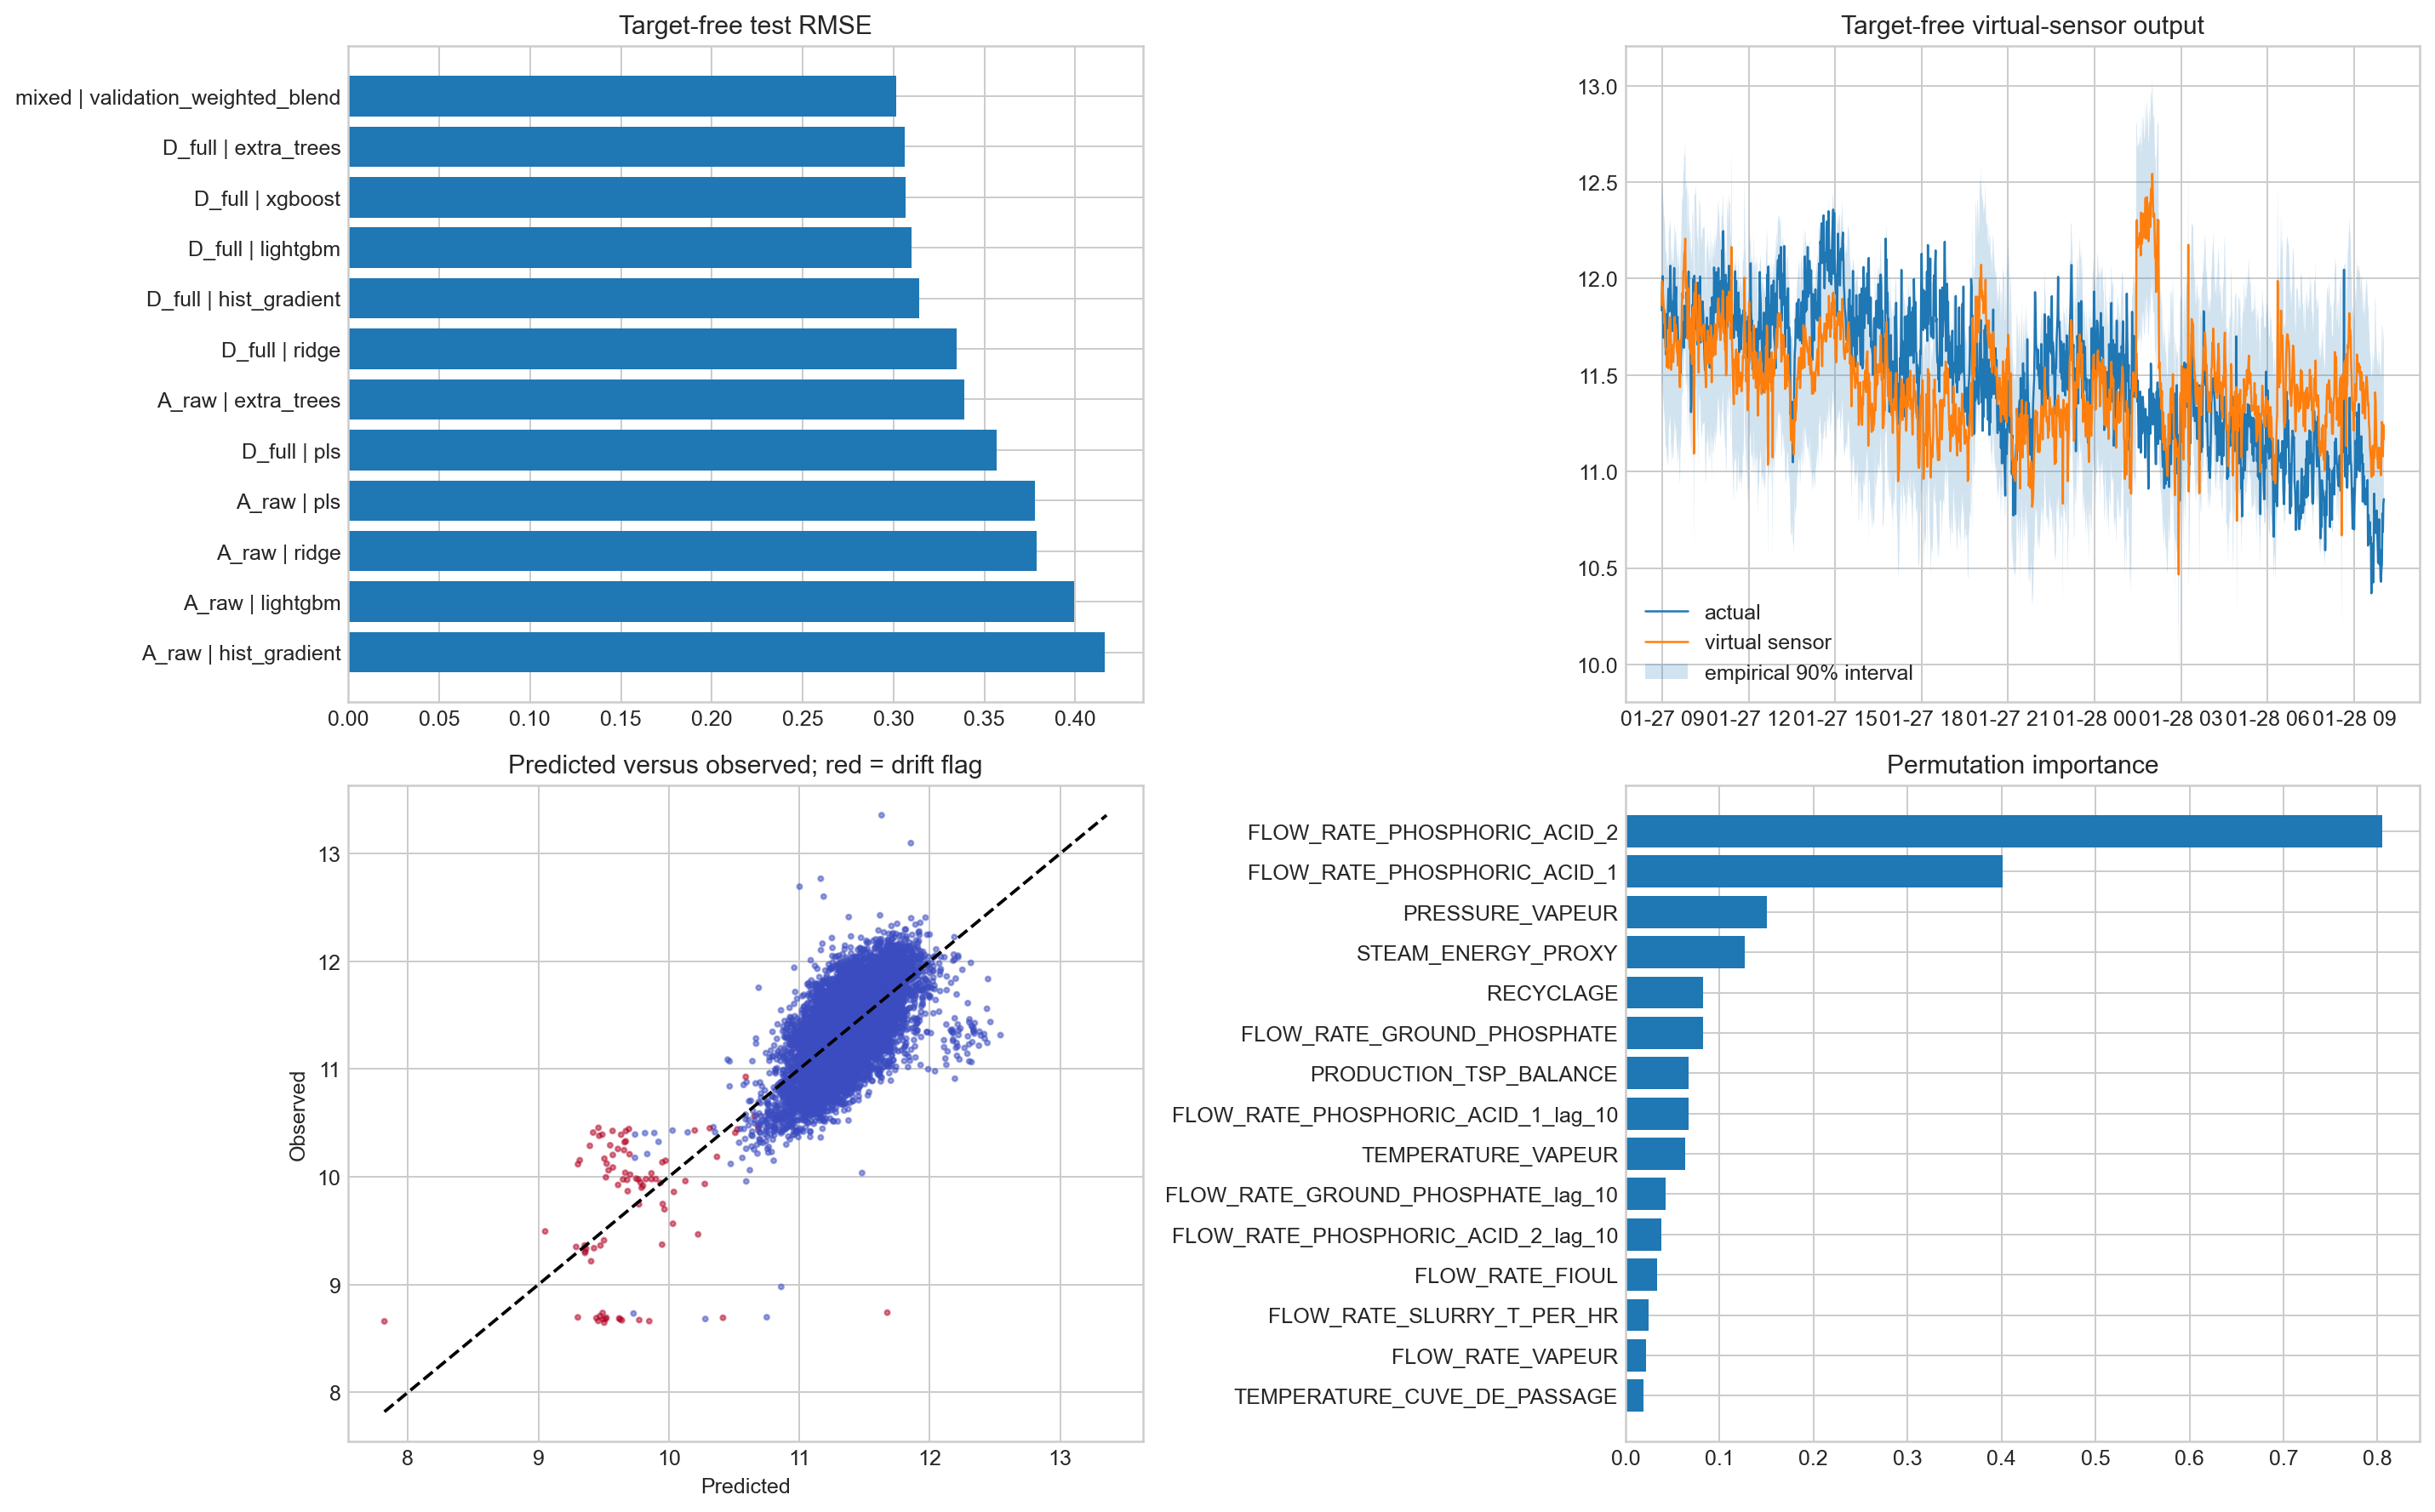
\includegraphics[width=0.82\textwidth]{exogenous_virtual_sensor_artifacts/figures/virtual_sensor_performance.png}
\caption{Target-free model comparison, example time series, predicted-versus-observed behavior, and validation permutation importance. Importance indicates association, not causality.}
\end{figure}

\begin{itemize}
  \item The empirical 90\% interval achieved 89.7\% test coverage with mean width 1.015.
  \item The drift score flags rows beyond the training 99th percentile.
  \item Only 1.37\% of test rows were flagged, but errors were substantially higher on those rows.
\end{itemize}

\textbf{Uncertainty limitation:} the interval width was calibrated from individual-Ridge validation residuals, while the final point estimate is a Ridge--LightGBM blend. I therefore treat it as an empirical diagnostic, not a formal coverage guarantee.

\section{Interactive dashboard}

I built the dashboard to make the notebook outputs usable without rerunning notebook cells. It supports:
\begin{itemize}
  \item default-month analysis or CSV upload;
  \item signal trajectories, missingness, pairwise relationship exploration, and dataset observations;
  \item candidate multivariate process-change windows and their main sensor drivers;
  \item later target response and prediction-error comparison when labels are available;
  \item target-anchored forecasts at 1, 5, 10, and 15 minutes;
  \item target-free virtual-sensor estimates, uncertainty bands, and drift flags;
  \item report generation and cached preprocessing/model loading.
\end{itemize}

\textbf{Important:} the green multivariate process-change score measures joint standardized sensor movement. It does not use future target change and does not confirm a startup, shutdown, fault, or abnormal target event.

\section{What is established and what is not}

\begin{tabularx}{\textwidth}{Y Y}
\toprule
\textbf{Supported by executed evidence} & \textbf{Not yet established} \\
\midrule
Chronological, leakage-controlled preparation across four horizons and four feature sets & Generalization to another month, season, product grade, or long-term sensor condition \\
Target-anchored delta forecasting beats persistence at every tested horizon & Operational warning performance during confirmed plant events \\
Temporal, process-aware, and target-history evidence provide measurable ablation gains & Causal influence or safe operator interventions \\
Target-free current-time estimation materially beats constant baselines & Target-free 5--15 minute early-warning performance \\
Input drift is associated with weaker prediction support & Guaranteed uncertainty coverage outside the observed training distribution \\
\bottomrule
\end{tabularx}

\section{Process-validation requirements}

I still need process-engineer confirmation for:
\begin{enumerate}
  \item Confirm units of phosphoric-acid flow, ground-phosphate flow, fuel-oil flow, steam flow, wash-liquid flow, and recyclage.
  \item Define the exact material or process stream represented by \texttt{RECYCLAGE}.
  \item Confirm whether \texttt{FLOW\_RATE\_SLURRY\_T\_PER\_HR} represents the same combined stream as total slurry volumetric flow.
  \item Identify confirmed startups, shutdowns, cleaning, maintenance, grade changes, and process disturbances.
  \item Confirm which variables are genuinely controllable before any what-if or intervention recommendation.
  \item Define acceptable prediction error, warning lead time, false-warning cost, and missed-event cost.
\end{enumerate}

\section{Recommended next work}

\begin{enumerate}
  \item \textbf{Freeze the current pipelines and test a later labeled month.} Report performance without retuning first; this is the highest-priority generalization test.
  \item \textbf{Validate regimes against plant records.} Replace statistical ``candidate'' labels with confirmed event categories where possible.
  \item \textbf{Recalibrate blend uncertainty.} Use out-of-sample blend residuals rather than individual-Ridge residuals.
  \item \textbf{Run rolling-origin validation across multiple months.} Repeatedly train on the past and predict the next chronological block.
  \item \textbf{Define the operational target.} Choose among current-time virtual sensing, target-anchored forecasting, and target-free future warning based on actual sensor availability.
  \item \textbf{Only then refine models.} Increase tuning budgets or test sequence models only if multi-month evidence shows a remaining, practically important gap.
\end{enumerate}

\section*{Current conclusion}

\statusbox{\textbf{What I have completed:} data exploration, leakage-controlled feature preparation, direct and delta forecasting benchmarks, transition diagnostics, a target-free virtual sensor, and an interactive dashboard. The hybrid Ridge is the strongest forecast when the current target is available. The Ridge--LightGBM blend is the strongest target-free current estimator so far.}

\end{document}
